\documentclass{beamer}

\usepackage{color}
\definecolor{keywordcolor}{rgb}{0.7, 0.1, 0.1}   % red
\definecolor{tacticcolor}{rgb}{0.0, 0.1, 0.6}    % blue
\definecolor{commentcolor}{rgb}{0.4, 0.4, 0.4}   % grey
\definecolor{symbolcolor}{rgb}{0.0, 0.1, 0.6}    % blue
\definecolor{sortcolor}{rgb}{0.1, 0.5, 0.1}      % green
\definecolor{attributecolor}{rgb}{0.7, 0.1, 0.1} % red

\usepackage{listings}
\def\lstlanguagefiles{lstlean.tex}
\lstset{language=lean}

\usepackage[T1]{fontenc}
\usepackage{amsmath, amssymb, upgreek}
\usepackage{stmaryrd}
\usepackage{bussproofs}
\usepackage{hyperref}
\usepackage{tikz}
\usepackage{unixode}

\newcommand{\ttt}[1]{\texttt{#1}}

\newcommand{\bN}{\mathbb{N}}
\newcommand{\bZ}{\mathbb{Z}}
\newcommand{\bR}{\mathbb{R}}
\newcommand{\Type}{\ttt{Type}}
\newcommand{\Prop}{\ttt{Prop}}
\newcommand{\fst}{\mathrm{fst}}
\newcommand{\snd}{\mathrm{snd}}
\newcommand{\letin}[3]{\mathrm{let}\ #1\ := #2\ \mathrm{in}\ #3}
\newcommand{\pair}[2]{\langle #1,\ #2\rangle}
\newcommand{\uPi}{\Uppi}
\newcommand{\lam}{\lambda}
\newcommand{\lx}{\lam x}
\newcommand{\ra}{\rightarrow}
\renewcommand{\th}{\vdash}
\newcommand{\sep}{\ \mid\ }
\newcommand{\subst}[2]{[#2/#1]}
\newcommand{\ueq}{\cong}
\newcommand{\I}[1]{\llbracket #1\rrbracket}
\newcommand{\mvar}{?\!}
\newcommand{\lean}{Lean}

\title{The Lean Theorem Prover}

\author{Cody Roux}

\begin{document}

\begin{frame}
  \maketitle
\end{frame}

\section{Overview}

\begin{frame}{What is theorem proving?}
  The field of Theorem Proving investigates expressing and proving
  \emph{mathematical theorems} with the help of computers

\end{frame}

\begin{frame}{What is it good for?}
  Any mathematical theorem is game, but one of the prime applications
  is verification of \emph{hardware and software applications.}
\end{frame}

\begin{frame}{What is it good for... in CS?}
  \begin{center}
    ``If you're dealing with life and death, consider proving some key
    algorithms. But in the real world, you arent gonna need it.'' --
    user RonJeffries, c2.com
  \end{center}
  \begin{center}
    ``[T]he absence of continuity, the inevitability of change, and
    the complexity of specification of significantly many real
    programs make the formal verification process difficult to justify
    and manage.'' -- De Millo, Lipton and Perlis, {\it Social
      Processes and Proofs of Theorems and Programs (1979)}
  \end{center}
  \begin{center}
    ``Unfortunately, there is a wealth of evidence that automated
    verifying systems are out of the question'' -- {\it ibid}
  \end{center}
  \begin{center}
    ``The amount of formal reasoning required to prove even the
    smallest programs is beyond the capacity of most of us.'' --
    anonymous user, c2.com
  \end{center}
\end{frame}

\begin{frame}{What is it good for... in CS?}
  But...
  \begin{center}
    ``The striking thing about our CompCert results is that the
    middleend bugs we found in all other compilers are absent. As of
    early 2011, the under-development version of CompCert is the only
    compiler we have tested for which Csmith cannot find
    wrong-code errors. This is not for lack of trying: we have devoted
    about six CPU-years to the task. The apparent unbreakability of
    CompCert supports a strong argument that developing compiler
    optimizations within a proof framework, where safety checks are
    explicit and machine-checked, has tangible benefits for compiler
    users.'' -- Yang {\it et al.}, {\it Finding and Understanding Bugs
      in C Compilers}
  \end{center}
\end{frame}

\begin{frame}{Some Milestones}
  In Math:
  \begin{itemize}
  \item The Four Color Theorem (2005, Coq) \emph{every map can be colored with at most four colors}
  \item The Prime Number Theorem (2005, Isabelle) \emph{the prime numbers grow like $n/\log(n)$}
  \item The Feit-Thompson Theorem (2012, Coq) \emph{every group of odd order is solvable}
  \item The Kepler Conjecture (2014, HOL) \emph{we know how to pack oranges}
  \end{itemize}
  In CS:
  \begin{itemize}
  \item Verification of the driverless Metro 14 line in Paris (1998, B-method)
  \item Verification of the CompCert C compiler (2009, Coq)
  \item Verification of the seL4 microkernel (2014, Isabelle)
  \item Many more!
  \end{itemize}
\end{frame}

\begin{frame}{But what about me?}
  Alright, enough sales pitch!\bigskip

  How can you get started with theorem proving?
\end{frame}

\begin{frame}{Lean}
  Ok, some more sales pitch:\bigskip

  In this talk, I'll be using a new theorem prover called Lean, develloped by
  \begin{itemize}
  \item Leo de Moura, at Microsoft Research
  \item Jeremy Avigad, Soonho Kong, Floris van Doorn at CMU
  \item And many others!
  \end{itemize}
\end{frame}
  
\section{The Core Components}

\begin{frame}{The core components}
  An Interactive Theorem Prover (ITP) is
  \begin{itemize}
  \item
    \begin{block}{A theorem prover:}
      It needs to be able to \emph{verify} fully detailed formal
      proofs of theorems. We call this the \emph{Kernel}
    \end{block}
  \item
    \begin{block}{Interactive}
      It needs to help the user provide such proofs. This is called
      the \emph{Elaborator} and \emph{Proof Engine}.
    \end{block}
  \end{itemize}
\end{frame}

\begin{frame}{The core components}
  Two silly examples:
  \begin{block}{The ideal prover}
    \begin{itemize}
    \item The kernel: Some implementation of a powerful logic that can express all abstractions.
    \item The proof engine: Just a \texttt{Prove} button!
    \end{itemize}
  \end{block}
  \begin{block}{The simplest prover}
    \begin{itemize}
    \item The kernel: some implementation of a simple logic, like First Order Logic.
    \item The engine: just a proof parser.
    \end{itemize}
  \end{block}
  \begin{block}{Reality}
    Somewhere in between.
  \end{block}
\end{frame}


\begin{frame}{The Kernel}
  The kernel is the most important \emph{trusted component}. We need
  \begin{itemize}
  \item A simple but expressive logic
  \item A trustworthy implementation
  \end{itemize}
  The ideal implementation:

  \begin{center}
    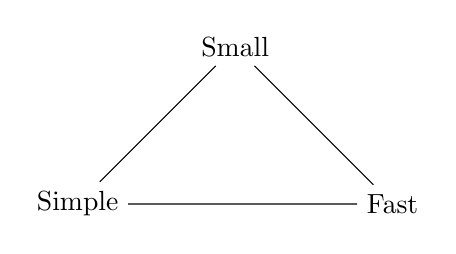
\begin{tikzpicture}
      
      
      \node (1) at (0,0) {Simple};
      \node (2) at (2,2) {Small};
      \node (3) at (4,0) {Fast};
      
      \draw[-] (1) -- (2) -- (3) -- (1);
    \end{tikzpicture}
  \end{center}


  Choose 2!
\end{frame}

\begin{frame}{The logic}
  We want simple (trustworthy, easy to implement) but powerful enough
  to formalize anything.
  \begin{block}{We use}
    \begin{itemize}
    \item A theory of \emph{dependent types} that unifies \emph{function
      spaces, universal quantifiers and polymorphism}
    \item A hierarchy of \emph{universes}
    \item Inductive families (GADTs in Haskell)
    \item Quotient types (useful to build $\mathbb{Z}$)
    \end{itemize}
  \end{block}
  This is similar to the logic of Coq.
\end{frame}

\begin{frame}{The implementation}
  \begin{itemize}
  \item Simple
  \item Very Fast
  \item In C++
  \item $\sim$ 6000 lines of code
  \end{itemize}

  There is an alternate implementation of the kernel, in Haskell (a
  couple thousand lines).
\end{frame}

\begin{frame}{A specification example}
  Let's work through an example to demonstrate the specification
  language:
  \begin{block}{Let's formalize the statement}
    There is an infinite number of primes.
  \end{block}
\end{frame}

\begin{frame}[fragile]{A specification example}
  First observation: logical connectives can be represented by
  inductive types
  \begin{lstlisting}
    inductive and (a b : Prop) : Prop :=
      intro : a → b → and a b

    inductive or (a b : Prop) : Prop :=
    | inl {} : a → or a b
    | inr {} : b → or a b

    inductive ⊤ : Prop := trivial : true

    inductive ⊥ : Prop

    definition ¬ (a : Prop) : Prop := a → ⊥

  \end{lstlisting}
  
\end{frame}
\begin{frame}[fragile]{A specification example}
  Even existence and equality
  \begin{lstlisting}
inductive Exists {A : Type} (P : A → Prop) : Prop :=
    intro : ∀ (a : A), P a → Exists P

    

inductive eq {A : Type} (a : A) : A → Prop :=
    refl : eq a a
  \end{lstlisting}
  
\end{frame}

\begin{frame}[fragile]{A specification example}
  Natural numbers are also spefied by induction
  \begin{lstlisting}
    inductive ℕ :=
    | zero : ℕ
    | succ : ℕ → ℕ
  \end{lstlisting}
  And operations are defined by recursion
  \begin{lstlisting}
    definition add : ℕ → ℕ → ℕ
    | add 0 m := m
    | add (succ n') m := succ (add n' m)

    definition mul : ℕ → ℕ → ℕ
    | mul 0 m := m
    | mul (succ n') m := add m (mul n' m)
  \end{lstlisting}
\end{frame}

\begin{frame}[fragile]{A specification example}
  with a few notations
  \begin{lstlisting}
    notation n `+` m := add n m
    notation n `*` m := mul n m
    ...
  \end{lstlisting}
  \begin{lstlisting}
    definition le (n m : ℕ) := ∃ k, n + k = m
    
    definition dvd (n m : ℕ) := ∃ k, n * k = m
    
    definition prime (p : ℕ) :=
    ∀ d, 2 ≤ p ∧ (d ∣ p → d = 1 ∨ d = p)
  \end{lstlisting}
  We can then express (and prove)
  
  \begin{lstlisting}
    theorem inf_primes := ∀ n, ∃ p, n ≤ p ∧ prime p
  \end{lstlisting}
\end{frame}

\begin{frame}[fragile]{The elaborator}
  To have any hope of being able to actually specify and prove
  anything, we need
  \begin{enumerate}
  \item a synthesizer for implicit arguments
    \begin{lstlisting}
 eq.subst : ∀ {A : Type}{a b : A}{P : A → Prop},
      a = b → P a → P b
    \end{lstlisting}
    we need to \emph{synthesize} (guess) values for $A, a, b$ and $P$!
    
  \item a language for proofs
  \end{enumerate}
\end{frame}

\begin{frame}[fragile]{The elaborator}
  This problem is non-obvious:
    \begin{lstlisting}
 eq.subst : ∀ {A : Type}{a b : A}{P : A → Prop},
      a = b → P a → P b
    \end{lstlisting}

    Say $P\ a\ \equiv\ a + a = 2$. Then we can have
    \[P\ \equiv\ \lambda x.\ x+x = 2\]
    or
    \[P\ \equiv\ \lambda x.\ x+a = 2\]
    \[P\ \equiv\ \lambda x.\ a+a = 2\]
    we need to account and search for \emph{multiple solutions}.
\end{frame}

\begin{frame}{The proof language}
  How to design an effective high-level proof language is one of the
  major open questions in ITP research.\bigskip

  Right now there are 2 main approaches:
  \begin{itemize}
  \item A ``stack based'' \emph{tactic language}, which operates by transforming the goal in a series of composable steps. Very powerful, but hard to read
  \item A declarative ``isar-like'' langauge, which is more verbose but easier to read and understand.
  \end{itemize}
  
  On top of this, we need some powerful proof automation to help with
  the simpler intermediate steps.
\end{frame}

\end{document}


